\section{Übungsaufgaben: Asymmetrische Kryptologie}
\subsection{Rucksack}
\subsection{RSA auf Nachricht in Blöcken}

\begin{align}
  P &= 'FHT4EVER'  &
  n &= 13 \cdot 17 = 221 & e &= 3
\end{align}

\begin{align}
	E(x) &=  x^3 \mod 221 \\
	E(P) &=  E('F') \circ E('H')\circ E('T')\circ E('4')\circ E('E')\circ E('V')\circ E('E')\circ E('R')\\
		 &=  [70, 72, 84, 52, 69, 86, 69, 82]     														\\
		 &=  [8, 200, 203, 52, 103, 18, 103, 194]
\end{align}


\subsection{chinesischer Restsatz}
\subsection{RSA-Low-Exponent-Attack}
\subsection{Quadratwurzeln mod n}
\subsection{Rabin}
\subsection{Elgamal}
\subsection{Diskrete Exponential-Funktion}
\subsection{Primfaktorzerlegung}
\subsection{Fermatscher Primzahltest}
\subsection{Inverses zu ($n-1) \mod n$}
\subsection{$a(n-1) \mod n$}
\subsection{$\phi(n)$ für $n < 500$}

\subsubsection{Berechnen Sie $\phi(n)$ für $n < 500$ und tragen Sie die Werte in einem Graphen}

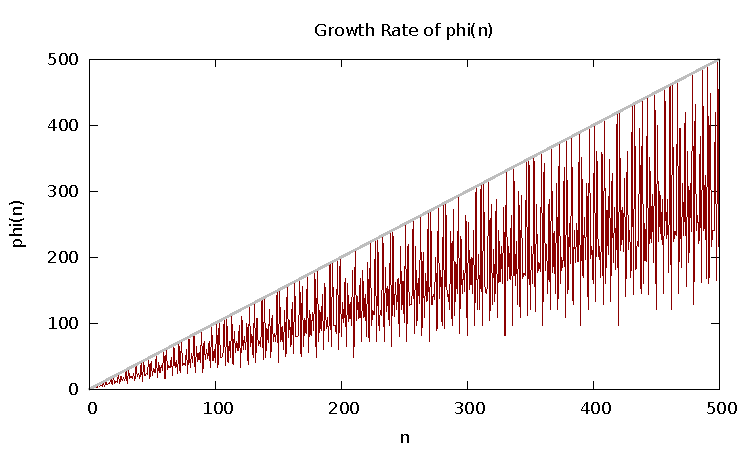
\includegraphics[scale=1]{eclipse/growth-rate.pdf}

\subsubsection{Geben Sie eine möglichst genaue obere Schranke für $\phi(n)$ an.}

\begin{align}
	 \phi(n) &\le n-1 \\
	 & \in \mathcal{O}(n)
\end{align}	
